\section{Problemas}

\subsection{Estimación de Pose en Humanos}

La tarea de \textit{Estimación de Pose en Humanos} ha sido uno de los tópicos de gran importancia en
el campo de Visión por Computadora. Debido a la búsqueda de automatización y entendimiento de
diversas actividades humanas, sus utilidades causan impacto directo en las implementaciones
tecnológicas del mundo real, tales como, la Predicción de Intención (vigilancia), Sistemas de
Autónomos y de Asistencia en la conducción automóviles, Animación, Simulaciones y Videojuegos
o hasta análisis de deportes. La tarea de \textit{Estimación de Pose} no solo se limita a el cuerpo
humano, también, puede ser empleado en objetos como carros o animales, vease la imagen ,


\begin{figure}[ht!]
    \centering
    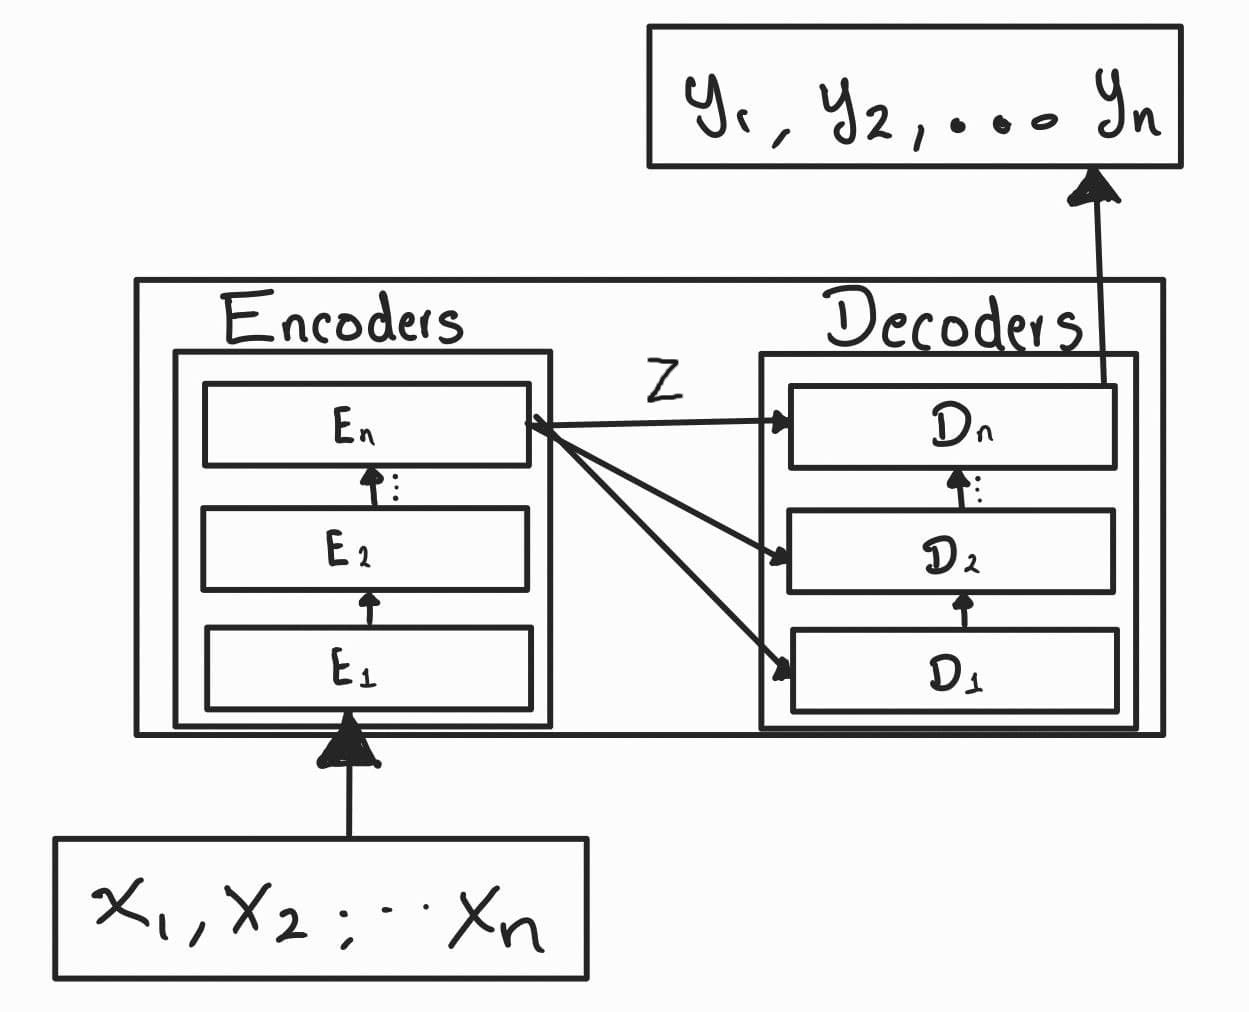
\includegraphics[width=0.4 \textwidth]{Chapters/2. Transformer/Figures/transformer/t_seq2seq.jpg}
    \caption{\cite{DBLP:journals/corr/abs-2103-02440}}
    \label{fig:trans_seq2sqe}
\end{figure}



Formally speaking, Pose Estimation is predicting the body part or joint positions of a person from
an image or a video.

The major challenges for tracking poses from the car perspective are
(i) occlusions due to the viewing angle and (ii) prediction
speed to be able to react to real-time changes in the environ

Problem Clasification by axes


- Number of People Being Tracked

Depending on the number of people being tracked, pose estimation can be classified into
Single-person and Multi-person pose estimation

Single-person pose estimation (SPPE) is the easier of the two, with the guarantee of only one person
present in the frame. On the other hand, Multi-person pose estimation (MPPE) needs to handle the
additional problem of inter-person occlusion. Initial approaches in pose estimation were mostly
focused on SPPE, however with the availability of huge multi-person datasets, the MPPE problem has
lately been getting increased attention.

- Input Modality

Red-Green-Blue (RGB) image : The images that we see around us on a daily basis, and the most common
type of input for Pose Estimation. Models working on RGB-only input have a huge advantage over
others in terms of the mobility of the input source. This is due to the ease of availability of
common cameras (which capture RGB images), making them the models that can be used across a huge
number of devices.

Depth (Time of Flight) image : In a Depth image, the value of a pixels relates to the distance from
the camera as measured by time-of-flight. The introduction and popularity of low-cost devices
like Microsoft Kinect has made it easier to obtain Depth data. Depth image can complement RGB image
to create more complex and accurate Computer Vision models, whereas Depth-only models are vastly
used where privacy is a concern.

Infra-red (IR) image : In an IR image, the value of a pixel is determined by the amount of infrared
light reflected back to the camera. Experimentation in Computer Vision based on IR images are minimal,
as compared to RGB and Depth images. Microsoft Kinect also provides IR image while recording.
However, currently there are no datasets that contain IR images.

Static Image vs Video

A video is nothing but a collection of images, where every two consecutive frames share a huge
portion of the information present in them (which is the basis of most of the video compression
techniques). These temporal (time based) dependence in videos can be exploited while performing
Pose estimation.
For a video, a series of poses need to be produced for the input video sequence. It is expected
that the estimated poses should ideally be consistent across successive frames of video, and the
algorithm needs to be computationally efficient to handle large number of frames. The problem of
occlusion might be easier to solve for a video due to the availability of past or future frames
where the body part is not occluded.

If temporal features are not a part of the pipeline, it is possible to apply static pose estimation
for each frame in a video. However, the results are generally not as good as desired due to jitters
and inconsistency problems.

2D vs 3D Pose Estimation

Depending on the output dimension requirement, the Pose Estimation problem can be classified into
2D Pose Estimation and 3D Pose Estimation. 2D Pose Estimation is predicting the location of body
joints in the image (in terms of pixel values). On the other hand, 3D Pose Estimation is predicting
a three-dimensional spatial arrangement of all the body joints as its final output.

2D Pose Estimation vs 3D Pose Estimation
Most 3D Pose Estimation models first predict 2D Pose, and then try to lift it to 3D Pose. However,
some end-to-end 3D Pose Estimation techniques also exist which directly predict 3D Pose.

Body Model
Every pose estimation algorithm agrees upon a body model beforehand. It allows the algorithm to formalize the problem of human pose estimation into that of estimating the body model parameters. Most algorithms use a simple N-joint rigid kinematic skeleton model (N is typically between 13 to 30) as the final output. Formally, kinematic models can be represented as a graph, where each vertex V represents a joint. The edges E can encode constraints or prior beliefs about the structure of the body model.
Such a model suffices for most applications. However, for many other applications such as character animation, a more elaborate model may be needed. Some techniques have considered a highly detailed mesh models, representing the whole body with a point cloud.
Another rather primitive body model that was used in earlier Pose Estimation pipelines is a shape-based body model. In shape-based models, human body parts are approximated using geometric shapes like rectangles, cylinders, conics etc.

kinematic Model
Planar Model
Volumetric Model
-> https://viso.ai/deep-learning/pose-estimation-ultimate-overview/

Number of cameras
A major portion of research involves solving the pose estimation problem using input from a single camera. However, there are certain algorithms which try to use data from multiple viewpoints/cameras, combining them to generate more accurate poses and handle occlusions better. The research on multi-camera pose estimation is currently somewhat limited, primarily due to lack of good datasets.

Why is it hard?
Strong articulations, small and barely visible joints, occlusions, clothing, and lighting changes make this a difficult problem.
Main challenges -> https://viso.ai/deep-learning/pose-estimation-ultimate-overview/

Pipelines

-> https://towardsdatascience.com/human-pose-estimation-simplified-6cfd88542ab3

Approaches

- Classical approaches
- Deep Learning based approaches
-> https://nanonets.com/blog/human-pose-estimation-2d-guide/
- Bottom-up
- Top-Down
-> https://viso.ai/deep-learning/pose-estimation-ultimate-overview/


Most popular pose estimation methods
-> https://viso.ai/deep-learning/pose-estimation-ultimate-overview/


\subsection{Lung Pathologies detection}
